\documentclass[11pt,pdftex,portrait,letterpaper]{article}
\usepackage[hdivide={1in,*,1in},
vdivide={1in,*,1in},
%            showframe
]{geometry}

% Standard packages
\usepackage[T1]{fontenc}
\usepackage{graphicx}
\usepackage{longtable}
\usepackage{acronym}
\usepackage{verbatim}
\usepackage{subfigure}
\usepackage{fancyhdr}
\pagestyle{fancy}
\usepackage{listings}
\usepackage{color}
\usepackage{lastpage}
\usepackage{caption}

% Fonts
%\usepackage{libertine}	% Libertine (the main font)
%\usepackage[lcgreekalpha]{libertinust1math}	% Libertine (as the math font)
\usepackage[varl]{inconsolata}	% A monospace font similar to Consolas. The varl option makes the lowercase l look different than a numeral 1.

% Last packages
\usepackage[hidelinks]{hyperref}	% Hyperlinks

% Modify parameters of Listings
\definecolor{lstgreen}{rgb}{0,0.6,0}
\definecolor{lstgray}{rgb}{0.4,0.4,0.4}
\lstset{ 
	language=C,
	basicstyle=\ttfamily\scriptsize,
	numbers=left,
	numberstyle=\footnotesize,
	keywordstyle=\color{blue},
	identifierstyle=\color{black},
	commentstyle=\color{lstgreen},
	stringstyle=\color{lstgray},
	stepnumber=1,
	numbersep=10pt,
	backgroundcolor=\color{white},
	frame=single,
	captionpos=b,
	breaklines=true,
	breakatwhitespace=false,
	tabsize=2,
	showstringspaces=false
}

% Default margins are too wide all the way around. Reset them here
\setlength{\topmargin}{-.5in}
\setlength{\textheight}{9in}
\setlength{\oddsidemargin}{0in}
\setlength{\textwidth}{6.5in}

\lhead{ECEN 220}
\chead{Project 4: Interrupt Service Routines}
\rhead{\thepage\ of \pageref{LastPage}}
\lfoot{\small{University of Nebraska--Lincoln}}
\cfoot{}
\rfoot{\small{Department of Electrical \& Computer Engineering}}
\renewcommand{\footrulewidth}{0.5pt}




\begin{document}
	
	\vspace*{30ex}
	\begin{center}
		
		\textbf{Project 4: Interrupt Service Routines}\\
		
		\vspace{4ex}
		ECEN 220: Introduction to Embedded Systems\\
		University of Nebraska--Lincoln\\
		April 7, 2021
		
		\vspace{4ex}
		Name: David Perez\\
		
	\end{center}
	
	
	\pagebreak
	\tableofcontents
	%\pagebreak
	%\listoffigures
	%\addcontentsline{toc}{section}{{\bf List of Figures}}
	\pagebreak
	
	
	\section{Introduction}
	
	During this project, we were tasked with experimenting with the timer/counter and ADC (analog to digital converter) peripherals. Alongside these peripherals, we used their ISR's (interrupt service routines) in order to be notified of when their task had complete rather then continuously read their registers flags like previous projects. This allowed us to not have to continuously check register values which consumes a lot energy and using infinite loops waiting for a register value change. 
	
	The interrupts for these two peripherals is pretty straight forward. The ISR for the ADC is triggered when the ADC conversion is complete, again allowing us to not devote our program to continuously checking its register conversion complete flag. The timer/counter ISR behaves similarly as it runs when the timer/counter has reached it's top value (which is declared in the OCR1AH and OCR1AL registers).
	
	With these ISR's we created two programs for this project. In the first one, we used the timer/coutner peripheral along with it's ISR to create a more accurate delay function relative to the one used in previous projects. In the second program we could use the delay generated by the timer/counter peripheral and create an appropriate delay to wait till our ADC would have completed a conversion, then perform an average of the 10 ADC temperature conversions. 
	
	
	\section{Program Description}
	
	For the first program in this project we were tasked with creating a delay using the timer/counter peripheral and it's ISR as stated above. In order to achieve this there were some key things to keep in mind. The first of which would be the timer/counter and specifically what prescalar and top value to use. Because we wanted a compare match every millisecond I concluded that I would need atleast a prescalar of 1. This was determined by using the following formula: prescalar >= f\_MCU / (f\_desired * 65536). Then, using the formula T(period) = TOP * prescsalar / f\_MCU  I got a value of 16,000. With this in mind I populated the timer/counter registers and put it in CTC mode and made sure it would not toggle PB1. 
	
	Next, I constructed my delay function that had a 32-bit parameter that would be used to set how long the delay would be when my delay function was called. Then, when the ISR was called it would decrement the milliseconds remaining variable. And finally the delay function would get out of it's infinite loop when there were 0 milliseconds remaining and  the ISR set the g\_myDelayDone to 1. After the delay had finished I would then toggle PB4 with a 25\% duty cycle.
	
	The second program contained just about everything from program 1 but it's task was to incorporate the delay function alongside the ADC peripheral. Some notable things from the ADC setup were the REFS bits in the ADMUX to set a 1.1v internal reference and the MUX bits which were set to 0b1000 to enable our temperature sensor. In the ADCSRA register I also set bit 3 to 1 to enable the ADC's ISR. Once I had this set up along with the timer/counter I also had to enable global interrupts and then start an infinite loop. In the loop I change bit 7 of ADCSRA to 7 to start the the ADC converion and delay for 100 milliseconds.
	
	Once the ADC's ISR completes it sets out global variable g\_adcDataReady to 1 indicating a completed conversion. Then I disable global interrupts to read the ADCL and ADCH registers, combine them into a 16bit value, then put that into a varible that contained all our ADC samples. If there had been 10 ADC samples I would divide the variable containg the summation of all our samples to find the average. Finally, I would print that vlaue to the serial monitor and reset all my variables and go back through the infinite loop.
	
	
	\subsection{Program 1}

	There are some other things pertaining to program 1 that I would also like to mention. Because this program uses interrupts there is a possibility that the interrupt will run when tyring to run an essential operation. For program 1 the section I deemed critical was when I was updating the g\_mSecsRemaining to be the same as the input parameter of my delay function. Also inside this crictical section I set the g\_myDelayDone variable to 0. Before and after these sections I disabled then re-enabled global interrupts to prevent them for causing errors in my program. Another key part to this program was creating the 25\% duty cycle by having a high time on pin PB4 for 1ms and a low time of 3ms resulting in a 4ms period (this is pictured in the figure below). 
	
	When using the timer/counter as a delay function I was able to achieve a fairly accurate delay. With a delay of 1ms I got a time of 1.02ms when read from the logic analyzer. With 50 insterted into myDelay function I got an actual delay of 49.99 ms. In comparison to my old delay function I obtained an actual delay of 1.04 for a 1ms delay and 50.144ms actual delay for a 50ms delay.I believe the reason behind the increased accuracy that the timer/counter pereipheral offers is due to the fact that you can use a much slower clock rate and make a percise counter. Using the MCU's clock on the other hand is extremely fast and inconcistent which results in greater inaccuracies when you increase the delay time. The timer/counter on the other hand is consistent with both 1 and 50 milliseconds.
	
	
	\begin{figure}[h]
		\centering
		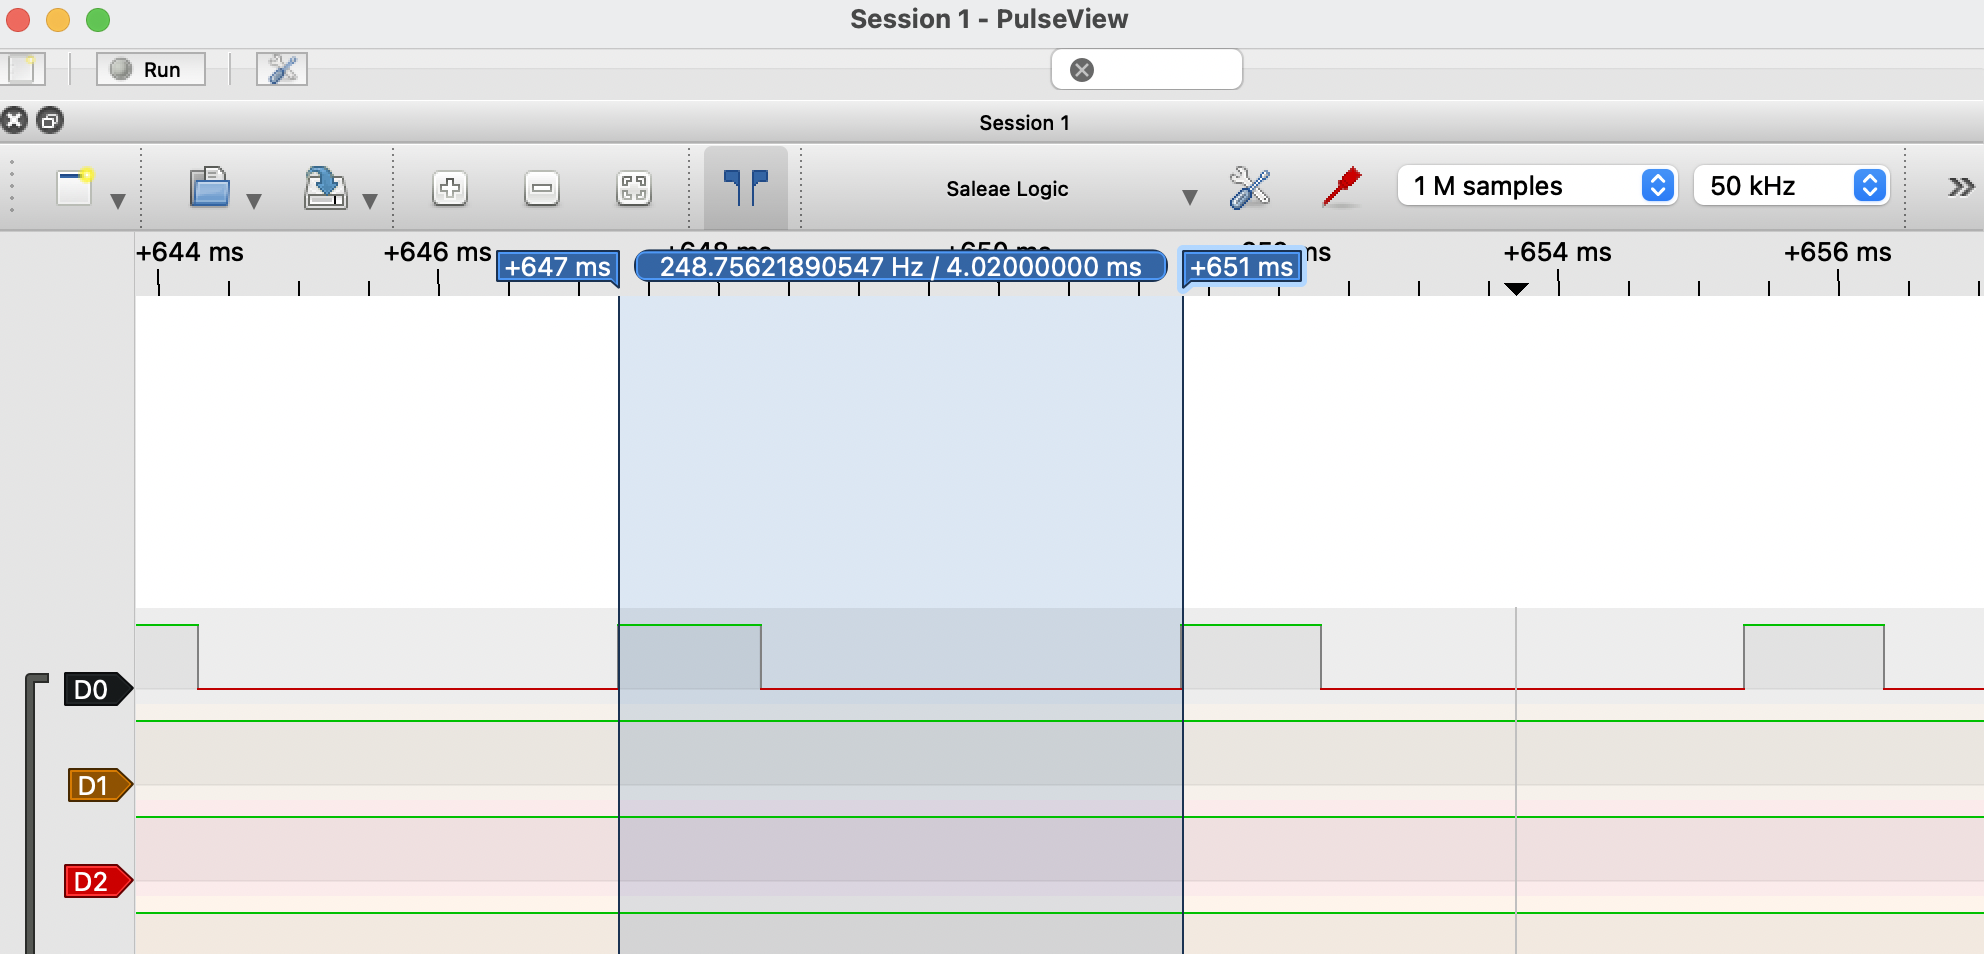
\includegraphics[width=0.80\textwidth]{./proj4_1ms}	% The .png file will be used to make the figure here, and is in the same directory as this .tex file
		\caption{25\% Duty Cycle with 4ms Period}
		\label{f:fig1}	% labels must come after the caption
	\end{figure}
	
	\pagebreak
	\subsection{Program 2}
	
	When creating program 2 there were a few sections I deemed critical and thus disabled then re-enabled global interrupts when performing these functions. The first critical section was when I was reading the register values in ADCL and ADCH, placing these into a 16-bit number, then putting this into my adcSamples variable which contained the summation of all the ADC conversions. Another critical section was when I calculated the average of the ADC samples, printed them to the serial monitor, and then reset my samples total and flag variables. And lasty, the final critical section was in myDelay function which sets the global variable g\_mSecsRemaining to the value in delayInMsec and sets g\_myDelayDone flag to 0.
	
	Upon running the program, the averaged value of the 10 ADC samples was around 328 give or take plus or minus 1 -2. I performed these measurements at a room temperature of 22 degrees celcius.Without actually converting the ADC value and simply comparing to the table from the datasheet where 25 degrees celcius gives and ADC value of 314 allowed me to assume I'm getting the right ADC readings considering the accuracy is +/- 10 degrees celcius.
	
	For this program there were a few ways to store and average the 10 ADC samples. The two that I could think of were storing them in an 16-bit array and dividing their total by 10 after there were 10 samples. The other method (the one that I used) was to put the 10 16-bit ADC voltages into a 32-bit varible then when there were 10 samples I'd divide that variable by 10 then print to ther serial plotter.
	
	
	
	
	\section{Conclusion}
	
	In program 1 and 2 in this project we were able to further our understanding of interrupts and also look back on the use of the ADC and timer/counter peripherals. In program 1 we used the timer/counter peripheral that called it's ISR on a compare match and would decrement the amount of miliseconds were remaining from the initial value given as a parameter to the myDelay function. This allowed for a more accurate delay function in comparison to previous projects and would get increasingly innacuraate when a longer delay time was used. In program 2 we used this delay to pause our prograam while we wait for an ADC conversion to complete and call it's ISR when it happened. We also set the ADC to use the internal temperature sensor to allow us to use our Arduino as a thermometer. All in all, we were able to better our understanding of the ADC and timer/counter peripherals and learn how to use their interrupts.
	
	\pagebreak
	
	
	\section{Appendix}
	
	%Here is an example of how to add good-looking code snippets using a 'listing' 
	\begin{lstlisting}[caption={Program 1}, label=l:programx]
		/** Includes **/
		#include <stdint.h>
		#include <avr/interrupt.h>
		
		/** Memory mapped register defines **/
		//Registers for GPIO pins
		#define REG_DDRB (*((volatile uint8_t*) 0x24))
		#define REG_PORTB (*((volatile uint8_t*) 0x25))
		
		//Registers for Timer/Counter peripheral
		#define REG_TCCR1A (*((volatile uint8_t*) 0x80))
		#define REG_TCCR1B (*((volatile uint8_t*) 0x81))
		#define REG_OCR1AH (*((volatile uint8_t*) 0x89))
		#define REG_OCR1AL (*((volatile uint8_t*) 0x88))
		#define REG_TCNT1H (*((volatile uint8_t*) 0x85))
		#define REG_TCNT1L (*((volatile uint8_t*) 0x84))
		
		//Interupt registers
		#define REG_TIMSK1 (*((volatile uint8_t*) 0x6F))
		#define REG_SREG   (*((volatile uint8_t*) 0x5F))
		
		/** Global Variables **/
		volatile uint32_t g_mSecsRemaining;
		volatile uint8_t g_myDelayDone;
		
		/** Defines **/
		#define BIT0  0X01
		#define BIT1  0X02
		#define BIT2  0X04
		#define BIT3  0X08
		#define BIT4  0X10
		#define BIT5  0X20
		#define BIT6  0X40
		#define BIT7  0X80
		
		/* Functions */
		void myDelay(uint32_t delayInMsec);
		
		int main()
		{
			/* Specifications:
			*  1.Use timer 1 in CTC mode to generate a "Timer 1 compare match" interrupt every 1 millisecond
			*  2.On a compare match call the Timer 1 compare match A ISR to decrement g_mSecsRemaining variable
			*    to create a delay for myDelay() function
			*  3. After the delay is done toggle pin PB4
			*/
			
			/*
			* Determine bit fields and relevant registers
			* Presclar >= f_MCU / (f_desired * TOP_max) == 16 MHz / (1000) * 65536) == .24414
			* 
			* WGM1[3:0] = 0b0100 for "Clear timer on Compare Match" (CTC)
			* mode, where the timer resets back to 0 when its value matches the output compare A registers OCR1A
			* COM1A[1:0] = 0b00, timer peripheral should not have control over pin OC1A/PB1
			* CS1[2:0] = 0b001 for a prescalar of 1
			* 
			* T = TOP * prescalar / f_MCU
			* OCR1A = TOP = T * f_MCU / prescalar == .001 * 16MHz / 1 == 16,000
			* 
			*/
			
			//Initialize global variables
			g_mSecsRemaining = 0;
			g_myDelayDone = 0;
			
			/* Set up Registers */
			//set PB4 as an output and initially low
			REG_DDRB |= BIT4;
			REG_PORTB &= ~BIT4; //clears only bit 4
			
			//Set the period using OCR1AH and OCR1AL
			const uint16_t TOP = 16000;
			REG_OCR1AH = TOP >> 8;
			REG_OCR1AL = TOP & 0x00FF;
			
			//TCCR1A contains COM1A[1:0] and WGM1[1:0]: COM1A[1:0] cat 0bxxxx cat WGM1[1:0] == 0b00 cat 0b0000 cat 0b00
			REG_TCCR1A = 0x00;
			
			//TCCR1B contains WGM1[3:2] and CS1[2:0] == 0b000 0b01 0b001
			REG_TCCR1B = 0x09;
			
			//Enable global interrupts in the SREG register
			REG_SREG |= BIT7;
			
			//Enable timer 1 compare match interrup in TIMSKI register
			REG_TIMSK1 |= BIT1;
			
			while(1)
			{
				//Turn PB4 low
				REG_PORTB &= ~BIT4;
				
				myDelay(3);
				
				//set PB4 High
				REG_PORTB |= BIT4;
				
				myDelay(1);
			}
		}
		
		void myDelay(uint32_t delayInMsec)
		{
			// Reset the Timer to 0
			REG_TCNT1H = 0x00;
			REG_TCNT1L = 0x00;
			
			//BEGINE CRITICAL SECTION OF CODE
			REG_SREG &= ~BIT7; // disable bit 7 (set to 0)
			
			//set our interupt milliseconds remaining value to the input to our delay function
			g_mSecsRemaining = delayInMsec; 
			//Also reset our delayDone flag to 0 in case it changed
			g_myDelayDone = 0;
			
			REG_SREG |= BIT7; //re enable global interrupts
			//END CRITICAL SECTION OF CODE
			
			while(g_myDelayDone != 1)
			{
				//Wait
			}
		}
		
		/** Interrupt Service Routines **/
		ISR(TIMER1_COMPA_vect, ISR_BLOCK)
		{
			//Decrement the number of miliseconds remaining
			g_mSecsRemaining--;
			
			//check if there are any milliseconds remaining
			if(g_mSecsRemaining == 0)
			{
				//this would mean there isn't any milliseconds remaining
				//so we set out indicatior to 1
				g_myDelayDone = 1;
			}
		}

	\end{lstlisting}
	
	\begin{lstlisting}[caption={Program 2}, label=l:programx]
		/** Includes **/
		#include <stdint.h>
		#include <avr/interrupt.h>
		
		/** Memory mapped register defines **/
		//Registers for Timer/Counter peripheral
		#define REG_TCCR1A (*((volatile uint8_t*) 0x80))
		#define REG_TCCR1B (*((volatile uint8_t*) 0x81))
		#define REG_OCR1AH (*((volatile uint8_t*) 0x89))
		#define REG_OCR1AL (*((volatile uint8_t*) 0x88))
		#define REG_TCNT1H (*((volatile uint8_t*) 0x85))
		#define REG_TCNT1L (*((volatile uint8_t*) 0x84))
		
		//Global variables for ADC registers
		#define REG_ADMUX  (*((volatile uint8_t*) 0x7C))
		#define REG_ADCSRA (*((volatile uint8_t*) 0x7A))
		#define REG_ADCL   (*((volatile uint8_t*) 0x78))
		#define REG_ADCH   (*((volatile uint8_t*) 0x79))
		
		//Interupt registers
		#define REG_TIMSK1 (*((volatile uint8_t*) 0x6F))
		#define REG_SREG   (*((volatile uint8_t*) 0x5F))
		
		/** Global Variables for delay function **/
		volatile uint32_t g_mSecsRemaining;
		volatile uint8_t g_myDelayDone;
		volatile uint32_t g_adcDataReady;
		
		
		/** Defines **/
		#define BIT0  0X01
		#define BIT1  0X02
		#define BIT2  0X04
		#define BIT3  0X08
		#define BIT4  0X10
		#define BIT5  0X20
		#define BIT6  0X40
		#define BIT7  0X80
		
		int main(void)
		{
			/* Specifications:
			*  1.Use timer 1 in CTC mode to generate a "Timer 1 compare match" interrupt every 1 millisecond
			*  2.On a compare match call the Timer 1 compare match A ISR to decrement g_mSecsRemaining variable
			*    to create a delay for myDelay() function
			*  3. After the delay is done togle pin PB4
			*/
			
			/*
			* Determine bit fields and relevant registers
			* Presclar >= f_MCU / (f_desired * TOP_max) == 16 MHz / (1000) * 65536) == .24414
			* 
			* WGM1[3:0] = 0b0100 for "Clear timer on Compare Match" (CTC)
			* mode, where the timer resets back to 0 when its value matches the output compare A registers OCR1A
			* COM1A[1:0] = 0b00, timer peripheral should not have control over pin OC1A/PB1
			* CS1[2:0] = 0b001 for a prescalar of 1
			* 
			* T = TOP * prescalar / f_MCU
			* OCR1A = TOP = T * f_MCU / prescalar == .001 * 16MHz / 1 == 16,000
			* 
			*/
			
			//Initialize global variables
			g_mSecsRemaining = 0;
			g_myDelayDone = 0;
			g_adcDataReady = 0;
			
			//initialize our flag indicating 10 adc conversions and our variable for holding adc samples
			uint8_t tenSamplesFlag = 0;
			uint32_t adcSamples = 0;
			
			/* Set up Registers for timer peripheral*/
			
			//Set the period using OCR1AH and OCR1AL
			const uint16_t TOP = 16000;
			REG_OCR1AH = TOP >> 8;
			REG_OCR1AL = TOP & 0x00FF;
			
			//TCCR1A contains COM1A[1:0] and WGM1[1:0]: COM1A[1:0] cat 0bxxxx cat WGM1[1:0] == 0b00 cat 0b0000 cat 0b00
			REG_TCCR1A = 0x00;
			
			//TCCR1B contains WGM1[3:2] and CS1[2:0] == 0b000 0b01 0b001
			// when the CS1 is no longer 0 the timer begins counting
			REG_TCCR1B = 0x09;
			
			//Enable timer 1 compare match interrup in TIMSKI register
			REG_TIMSK1 |= BIT1;
			
			//Enable global interrupts in the SREG register
			REG_SREG |= BIT7;
			
			/** Set up ADC peripheral registers **/
			//REFS[1:0] = 0b11 for internal 1.1v reference
			//ADLAR(bit 5) = 0b0 to be "right adjusted"
			// bit 4 of mux == 0b0 (un-used bit)
			//MUX[3:0] = 0b1000 (to enable temperature sensor)
			//concate bits, ADMUX == 0b 1100 1000
			REG_ADMUX = 0xC8;
			
			/* Next, configure the ADCSRA register */
			//ADEN = 0b1 to enable ADC
			//ADSC = 0b0 so that that we don't start conversion early
			//bits 5 4 we ignore and set to 0's
			//bit 3 = 0b1 to enable adc interrupt
			// ADPS[2:0] = 0b111 to select the prescalar division ratio as 128
			// so that (16Mhz / 128 = 125Khz, which is in between 50 and 200khz as per spec
			//concat and place in ioADCSRA == 0b 1000 1111 == 0x
			REG_ADCSRA = 0x8F;
			
			while(1)
			{
				/* Start the ADC conversion */
				//To do this, we need to set ADSC (this is bit 6 of the
				//ADCSRA register) to a 0b1
				//Read-write-modify
				REG_ADCSRA |= 0x40;  // same as line above
				
				//Delay for 100ms
				myDelay(100);
				
				if(g_adcDataReady == 1)
				{
					//BEGIN CRITICAL SECTION OF CODE
					REG_SREG &= ~BIT7; // disable bit 7 (set to 0)
					
					//The ADC conversion has completed!
					//Now read the ADC value
					//Read ADCL register first
					uint8_t adc_low_value = REG_ADCL;
					
					//Now, read the ADCH register
					uint8_t adc_high_value = REG_ADCH;
					
					//combine the high and low value into a single 16 usigned integer
					uint16_t adcResult = adc_low_value & 0x00FF;
					adcResult = (adcResult) | ((uint16_t)adc_high_value << 8);
					
					//store our 16-bit adc value in a 32-bit to hold all our adc values
					uint32_t adcSamples = adcSamples + adcResult; 
					
					REG_SREG |= BIT7; //re enable global interrupts
					//END CRITICAL SECTION OF CODE 
					
					//reseting our flag that indiactees a completed adc conversion
					g_adcDataReady = 0;
					
					//increment our flag indicating 10 samples
					tenSamplesFlag++;
					
					// If we have 10 adc samples we're going to print the average of them
					if(tenSamplesFlag == 10)
					{
						
						//BEGIN CRITICAL SECTION OF CODE
						REG_SREG &= ~BIT7; // disable bit 7 (set to 0)
						
						//find the average of our adc samples
						uint32_t adcAverage = adcSamples / 10;
						
						//begin serial transmission and print our adc average
						Serial.begin(9600);
						
						//           char message[80];
						//           sprintf(message,"ADC value %u \n",adcAverage);
						//           Serial.write(message);
						Serial.println(adcAverage);
						
						
						
						adcAverage = 0;
						adcSamples = 0;
						
						REG_SREG |= BIT7; //re enable global interrupts
						//END CRITICAL SECTION OF CODE 
						
						//reset our flag back to 0
						tenSamplesFlag = 0;
					}
				}
			}
		}      
		
		
		void myDelay(uint32_t delayInMsec)
		{
			// Reset the Timer to 0
			REG_TCNT1H = 0x00;
			REG_TCNT1L = 0x00;
			
			//BEGINE CRITICAL SECTION OF CODE
			REG_SREG &= ~BIT7; // disable bit 7 (set to 0)
			
			//set our interupt milliseconds remaining value to the input to our delay function
			g_mSecsRemaining = delayInMsec; 
			//Also reset our delayDone flag to 0 in case it changed
			g_myDelayDone = 0;
			
			REG_SREG |= BIT7; //re enable global interrupts
			//END CRITICAL SECTION OF CODE
			
			while(g_myDelayDone != 1)
			{
				//Wait
			} 
		}
		
		/** Interrupt Service Routines **/
		
		//ISR for Timer used by delay function
		ISR(TIMER1_COMPA_vect, ISR_BLOCK)
		{
			//Decrement the number of miliseconds remaining
			g_mSecsRemaining--;
			
			//check if there are any milliseconds remaining
			if(g_mSecsRemaining == 0)
			{
				//this would mean there isn't any milliseconds remaining
				//so we set out indicatior to 1
				g_myDelayDone = 1;
			}
		}
		
		//ISR fires when an adc conversion completes
		ISR(ADC_vect, ISR_BLOCK)
		{
			//Set data flag to 1 indicating ADC conversion is complete and new data available
			g_adcDataReady = 1;
		}
	
		
	\end{lstlisting}
	
	
	
	
\end{document}



